\documentclass{scrreprt}

%Für deutsche Trennung
\usepackage[ngerman]{babel}
%Für UTF8-Codierung, mit Umlauten!
\usepackage[utf8]{inputenc}

%Für Links, auch innerhalb des Dokuments
\usepackage{hyperref}

%Einbinden von Grafiken
\usepackage{graphicx}

\title{Anwenden der Patterns}
\author{Gruppe H}
\date{\today}

\begin{document}

\maketitle
\tableofcontents

\part{Welches Pattern eignet sich für unseren Faithinator?}

\chapter{Broker}
Das Broker-Pattern eignet sich nicht für den Faithinator, da es in der Praxis aus gutem Grund überwiegend für verteilte Systeme (“distributed systems”) verwendet wird. Das Broker-Pattern ist äußerst komplex und bietet beispielsweise eine hohe Redundanz, die für unsere App nicht benötigt wird. Aufgrund der Komplexität und des begrenzten zeitlichen Rahmens unseres Programmierpraktikums ist davon also abzuraten. Außerdem wollen wir kein verteiltes Softwaresystem entwickeln, sondern eine handelsübliche Android App.

\chapter{Blackboard}
Das Blackboard-Pattern eignet sich wunderbar zur Lösung von komplexen Problemen (wie z.B. Spracherkennung), da es, bildlich gesprochen, das Problem in Teilprobleme aufteilt, die parallelisiert abgearbeitet werden können. In Bezug auf unseren Faithinator ist aber auch dieses Pattern äußerst ungeeignet, da es keine solch komplexen Probleme zu lösen gilt und eine Benutzer-Interaktive Anwendung entwickelt werden soll.

\chapter{Presentation-Abstraction-Control}
Das PAC - Pattern eignet sich gut zur Implementierung der App. Der Top-Level Agent überwacht die Datenbank, die Bottom-Level Agents sind für die Benutzeroberfläche zuständig (Präsentation von Ergebnissen, Darstellung der Fragen etc. ). Die App erfordert eine hohe Kommunikation zwischen User und System und das macht das PAC - Pattern unkompliziert möglich.
\begin{figure}[ht]
 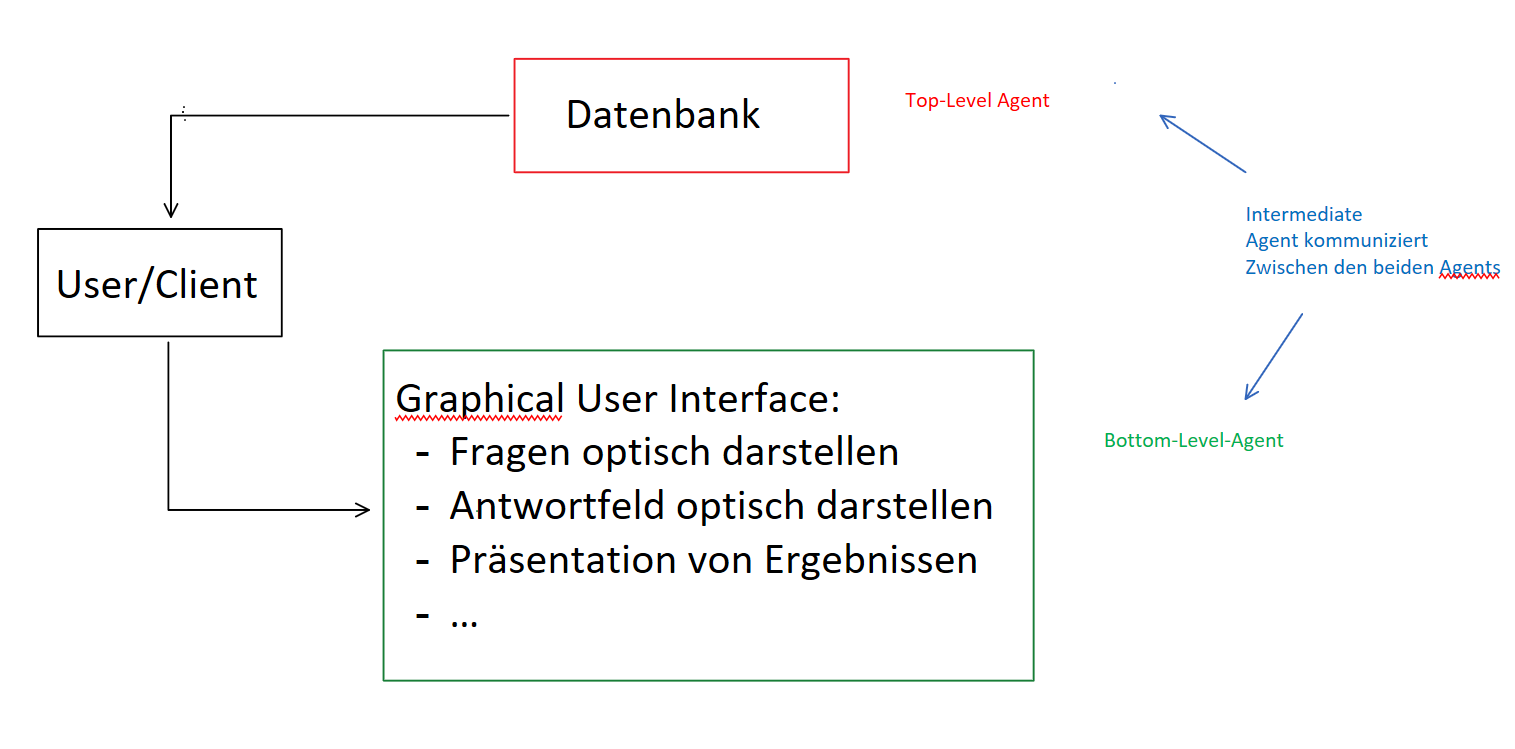
\includegraphics[width=\textwidth]{./pics/PAC.PNG}
 % Diagramm1e.eps: 0x0 pixel, 300dpi, 0.00x0.00 cm, bb=0 0 765 425
 \caption{Übersicht: Zusammenarbeit der Komponenten}
 \label{abb:1}
\end{figure}

\chapter{Model-View-Controller}
Auch das MVC -  Pattern kann zur Implementation der App verwendet werden. Die drei Komponenten des MVC - Pattern sind Modell, Präsentation und Steuerung. Das Modell im Fall des Faithinator sei die Datenbank, die sämtliche Informationen enthält. Die Präsentationsschicht stellt diese Daten dar (in unserem Fall die Fragen und Antworten). Da die App auf Benutzeraktionen basiert, ist die Steuerung ebenfalls wichtig.
\begin{figure}[ht]
 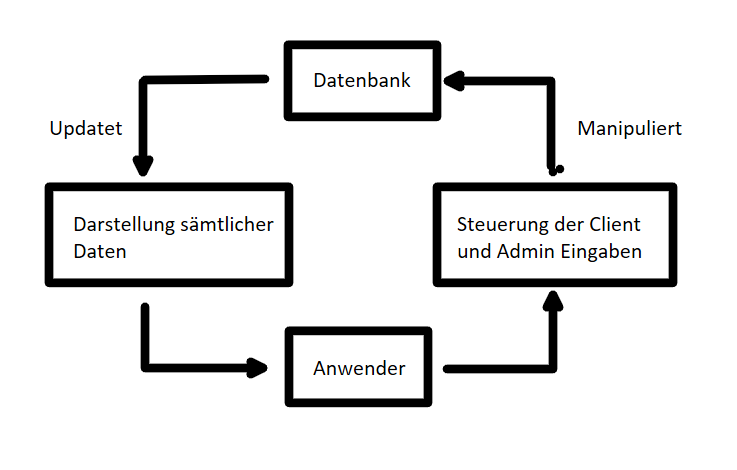
\includegraphics[width=\textwidth]{./pics/MVC.PNG}
 % Diagramm1e.eps: 0x0 pixel, 300dpi, 0.00x0.00 cm, bb=0 0 765 425
 \caption{Übersicht: Zusammenarbeit der Komponenten}
 \label{abb:2}
\end{figure}

\chapter{Pipes and Filters}
Das Pipes and Filters - Pattern benötigt man nicht für die Implementierung des Faithinators. Die Pipes and Filters werden normalerweise verwendet um eingehende Datenströme zu verarbeiten. In unserem Fall wollen wir eingehende Daten wie Registrierungsdaten nur speichern und benötigen keine weitere Verarbeitung. Auch für die Antworten, die die Clients geben wollen wir eigentlich nur in die Datenbank schreiben.
\chapter{Reflection}
Es wäre sinnvoll das Reflection-Pattern bei der Implementierung des Faithinators zu nutzen. Das Reflection-Pattern ist nützlich um nachträglich noch Dinge zu ändern und das möglichst kostengünstig und effizient. In unserem Fall bietet sich dies an um den Faithinator immer auf dem aktuellen Stand zu halten und nachträglich noch zusätzliche Funktionen einzubauen. Das würde nur theoretisch nach dem  Praktikum passieren.

\chapter{Layers Pattern}
Als Beispiel für das Layering typischer Software wird in der Literatur (Buschmann, S. 38) folgender Aufbau genannt:

\begin{quote}
\begin{itemize}
 \item User-visible elements
 \item Specific application modules
 \item Common service level
 \item Operating system interface level
 \item Operating system
 \item Hardware
\end{itemize}
\end{quote}

Betrachtet man die Android-App für sich, so stellt man fest, dass die Umgebung für Android Programmierung, die eng mit dem Betriebssystem Android verbunden ist, bereits eine solche Layerstruktur darstellt. Es existiert ein umfangreiches System aus Klassen und Methoden, die einen einfachen, weil durch mehrere Schichten abstrahierten Zugang über Programmierschnittstellen (APIs) ermöglicht. Die Schichten 3-6 werden bereits durch Android Studio abgedeckt. Die Kommunikation zwischen den Schichten wird auch seitens Android Studio unterstützt.

Das Pattern ist in erster Linie für Systeme mit einer großen “Tiefe” gedacht, die vom Userinterface bis zur Hardware reicht. Wir werden dieses Pattern passiv verwenden, indem wir die durch die Java Virtual Machine und Android bereit gestellten Strukturen nutzen, die dieses Prinzip so konsequent und erfolgreich umgesetzt haben, dass sogar am Gesamtsystem unbeteiligte wie wir, erfolgreich damit arbeiten können. Die Zielvorgabe, dass es so klare Grenzen zwischen den Strukturen gibt, dass Komponenten in den Schichten ausgetauscht werden können und das System lauffähig bleibt, wurde erreicht.
Die uns verbleibenden Zuständigkeiten haben eine sehr geringe übrige “Tiefe”, so dass eine weitere Aufteilung in Schichten wenig sinnvoll erscheint, bzw. die horizontalen Schichten so wenige sind und der vertikale Strukturierungsbedarf im Vergleich dazu so hoch, dass die Struktur durch andere Pattern, besser beschrieben werden kann.

\chapter{Microkernel}

\end{document}
